%\documentclass[aps,prb,reprint,twocolumn,superscriptaddress,floatfix,10pt,letterpaper,showpacs]{revtex4-1}
%\usepackage{amsmath,amssymb,amsfonts,stmaryrd,wasysym,graphicx,multirow,color,textcomp}
%\usepackage{url}%\usepackage{diagrams}
%\usepackage[colorlinks=true,citecolor=blue,urlcolor=blue]{hyperref}

\newcommand{\TPf}{\hyperlink{TPf}{$\mathcal{T}$-$\mathrm{Pf}^\ast$} }


\subsection{\label{sec:Intro}Introduction}
Conventional topological insulators (\hypertarget{TI}{TI})~\cite{FuKaneMele3D,Roy07,MooreBalents07,QiHughesZhang08} are time reversal and charge $U(1)$ symmetric electronic band insulators in three dimensions that host massless surface Dirac fermions. The topologically protected surface Dirac fermion can acquire a single-body ferromagnetic or superconducting mass by breaking time reversal or charge $U(1)$ symmetry respectively, as described in the introduction chapter. Alternatively it can acquire a many-body interacting mass while preserving both symmetries, and exhibit long-ranged entangled surface topological order~\cite{WangPotterSenthilgapTI13,MetlitskiKaneFisher13b,ChenFidkowskiVishwanath14,BondersonNayakQi13}. Interfaces between different massive surface domains host exotic massless quasi-$(1+1)$D electronic channels~\cite{TeoKane,FuKanechargetransport09,QiWittenZhang13}, and consequently, from the bulk-boundary correspondence, topological insulator slabs with distinct gapped surface orders lead to a variety of quasi-$(2+1)$D topological phases. 
On the other hand, fractional topological insulators (\hypertarget{FTI}{FTI})~\cite{MaciejkoQiKarchZhang10,SwingleBarkeshliMcGreevySenthil11,maciejko2012models,ye2016composite,maciejko2015fractionalized,stern2016fractional,YeChengFradkin17} are long-range entangled topologically ordered electronic phases in $(3+1)$ dimensions outside of the single-body mean-field band theory description. They carry fractional quasi-particle and quasi-string excitations that cannot be adiabatically connected to the electron. 
They carry time reversal and charge $U(1)$ symmetries, which enrich its topological order (local excitation spectrum) in the sense that a symmetric surface must be anomalous and cannot be realized non-holographically by a true $(2+1)$-D system. In this paper, we describe the topological properties of various massive surface states and quasi-$(2+1)$-D slabs of a series of a fractional topological insulator. In particular, we focus on the quasi-particle structure.

\begin{figure}[htbp]
\centering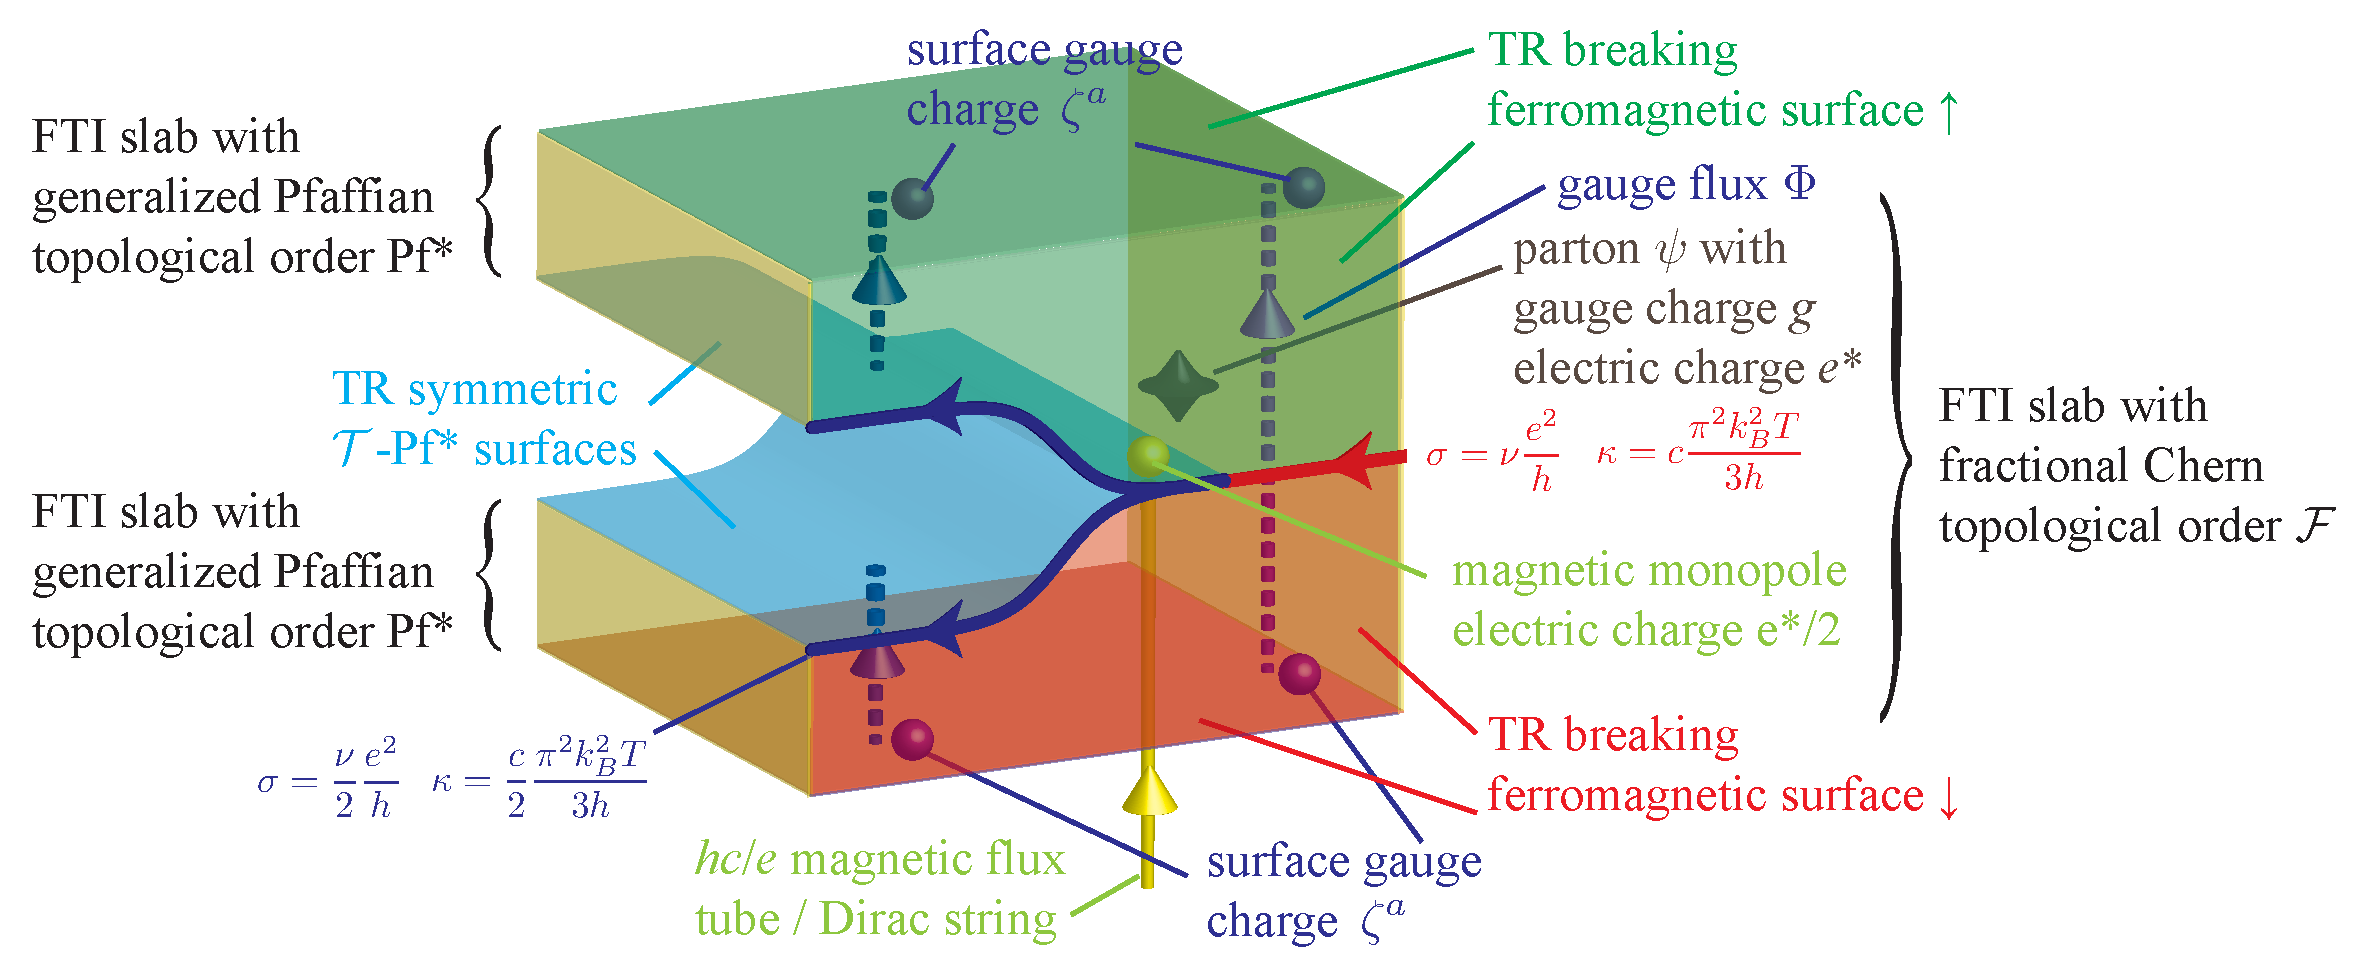
\includegraphics[width=0.9\textwidth]{fig1}
%\caption{Summary of the \QP and gauge flux content in \FTI slabs. A pair of $\mathrm{Pf}^\ast$ \FTI slabs are merged into a fracional Chern \FTI slab $\mathcal{F}$ by gluing the two \TR symmetric \TPf surfaces. Directed bold lines on the front surfaces are chiral edge modes of the $\mathrm{Pf}^\ast$ and $\mathcal{F}$ \FTI slabs.}\label{fig1}
\caption{Summary of the quasiparticle and gauge flux content in fractional topological insulator slabs. A pair of $\mathrm{Pf}^\ast$ fractional topological insulator slabs are merged into a fractional Chern insulator slab $\mathcal{F}$ by gluing the two time reversal symmetric $\mathcal{T}$-$\mathrm{Pf}^\ast$ surfaces. Directed bold lines on the front surface are chiral edge modes of the $\mathrm{Pf}^\ast$ and $\mathcal{F}$ fractional topological insulator slabs.}\label{fig1}
\end{figure}

We focus on a series of fermionic fractional topological insulators, labeled by integers $n$, whose magneto-electric response is characterized by the $\theta$-angle $\theta=\pi/(2n+1)$ (modulo $2\pi/(2n+1)$) that associates an electric charge of $e^\ast/2=e/2(2n+1)$ to each magnetic monopole~\cite{Witten79}, for $e$ the electric charge of the electron. In particular, we consider fractional topological insulators that support deconfined fermionic parton excitations $\psi$ in the bulk, each carrying a fractional electric charge of $e^\ast=e/(2n+1)$. This assumes the electron can be written as 2n+1 parts, i.e.  $\psi_{\mathrm{el}}\sim\psi_1\ldots\psi_{2n+1}$. The $(3+1)$-D topological order is based on a discrete $\mathbb{Z}_{2n+1}$ gauge theory~\cite{maciejko2012models}. This is necessary because these particles do not exist outside of the insulator, and so must glue together. This gauge theory ensures that, and there are several ways to do this but we just consider one.  The theory supports electrically neutral string-like gauge flux $\Phi$, so that a monodromy quantum phase of $e^{2\pi ig/(2n+1)}$ is obtained each time $\psi$ orbits around it. In other words, $\psi$ carries the gauge charge $g$ that braids with the gauge flux. The integer $g$ and $2n+1$ are relatively prime so that all local quasiparticles be combinations of the electronic quasiparticles $\psi_{\mathrm{el}}$ and hence must carry integral electric charges and trivial gauge charges.

Generalizing the surface state of a conventional topological insulator, the surface of a fractional topological insulator hosts massless Dirac partons coupling with a $\mathbb{Z}_{2n+1}$ gauge theory. These anyons are bosons. Unlike its non-interacting counterpart whose gapless Dirac surface state is symmetry protected in the single-body picture, a fractional topological insulator is strongly interacting to begin with and there is no topological reason for its surface state to remain gapless. In this paper we focus on three types of gapped surface states -- ferromagnetic surfaces that break time reversal, superconducting surfaces that break charge $U(1)$, and symmetric surfaces which generalize the $\mathcal{T}$-Pfaffian surface state of a conventional topological insulator and is denoted by {$\mathcal{T}$-$\mathrm{Pf}^\ast$}. The topological order for fractional topological insulator slab with these surfaces are discussed in Sec.~\ref{FS}, \ref{SCS} and \ref{TPF} respectively. In Sec.~\ref{Gluing}, we discuss, using an anyon condensation picture, the gluing of a pair of $\mathcal{T}$-Pfaffian surfaces. We conclude in Sec.~\ref{Conclusion} with remarks on a complementary way to understand these topological order \cite{ChoTeoFradkin17}.
\subsection{\label{FS}Ferromagetic Heterostructure}
We begin with a slab that has opposite time reversal breaking ferromagnetic surfaces. In the ferromagnetic surfaces, in addition to the single-body Dirac mass $m$ for the surface parton, the $\mathbb{Z}_{2n+1}$ gauge sector also shows a time reversal breaking signature. The $\mathbb{Z}_{2n+1}$ gauge theory is only present inside the fractional topological insulator, and when a flux line $\Phi$ terminates at the surface, the time reversal breaking boundary condition confines an electrically neutral surface gauge quasiparticle, denoted by $\zeta^a$, with gauge charge $a$ at the flux-surface junction (see Fig.~\ref{fig1}). This gauge flux-charge composite, referred to as a dyon $\delta=\Phi\times\zeta^a$, carries fractional spin $h_\delta=a/(2n+1)$ because a $2\pi$-rotation about the normal axis braids $a$ gauge charges around $\Phi$ and results in the monodromy quantum phase of $e^{2\pi ia/(2n+1)}$. Time reversal conjugates all quantum phases so, $a\not\equiv0$ modulo $2n+1$ breaks time reversal.

The one-dimensional interface between two time reversal conjugate ferromagnetic surface domains hosts a fractional chiral channel. For example, the interface between two ferromagnetic domains with opposite ferromagnetic orientations on the surface of a conventional topological insulator bounds a chiral Dirac channel~\cite{TeoKane,FuKanechargetransport09,QiWittenZhang13}, where electrons propagate only in the forward direction. Alternatively, a topological insulator slab with opposite time reversal breaking ferromagnetic surfaces is topologically identical to a quasi-$(2+1)$-D Chern insulator~\cite{Haldane1988,liu2016quantum} and supports a chiral Dirac edge mode. Similarly, in the fractional topological insulator case, the low-energy content of the fractional chiral channel between a pair of time reversal conjugate ferromagnetic surface domains can be inferred by the edge mode of a fractional topological insulator slab with time reversal breaking ferromagnetic surfaces that is topologically identical to a quasi-$(2+1)$-D fractional Chern insulator~\cite{RegnaultBernevigfractionchern,NeupertSantosChamonMudry11,TangMeiWen11,ShengGuSunSheng11} or fractional quantum Hall (\hypertarget{FQH}{FQH}) state~\cite{FQHE_Review}. The chiral $(1+1)$-D channel is characterized by two response quantities~\cite{Laughlin_IQHE, Halperin82, Hatsugai93, Schulz00, Volovik92, KaneFisher97, Cappelli01, Kitaev06, Luttinger64} -- the differential electric conductance $\sigma=dI/dV=\nu e^2/h$ that relates the changes of electric current and potential, and the differential thermal conductance $\kappa=dI_T/dT=c(\pi^2k_B^2/3h)T$ that relates the changes of energy current and temperature. In the slab geometry, they are equivalent to the Hall conductance $\sigma=\sigma_{xy}$, $\kappa=\kappa_{xy}$. $\nu=N_e/N_\phi$ is also referred to as the filling fraction of the fractional topological insulator slab and associates the gain of electric charge (in units of $e$) to the addition of a magnetic flux quantum $hc/e$. $c=c_R-c_L$ is the chiral central charge of the conformal field theory (\hypertarget{CFT}{CFT})~\cite{bigyellowbook} that effectively describes the low-energy degrees of freedom of the fractional chiral channel. 

Since the top and bottom surfaces of the fractional topological insulator slab are time reversal conjugate, their parton Dirac masses $m$ and gauge flux-charge ratio $a$ have opposite signs. The anyon content is generated by the partons and gauge dyons. When a gauge flux passes through the entire slab geometry from the bottom to the top surface, it associates with total $2a$ gauge charges at the two surface junctions. We denote this dyon by $\gamma=\Phi\times\zeta^{2a}$, which corresponds to an electrically neutral anyon in the slab with spin $h_\gamma=2a/(2n+1)$. If $a$ is relatively prime with $2n+1$, the primitive dyon generates the chiral Abelian topological field theory $\mathbb{Z}_{2n+1}^{(2a)}$~\cite{MooreSeiberg89,Bondersonthesis}, which consists of the dyons $\gamma^m$, for $m=0,\ldots,2n$, with spins $h_{\gamma^m}=2am^2/(2n+1)$ modulo 1 and fusion rules $\gamma^m\times\gamma^{m'}=\gamma^{m+m'}$, $\gamma^{2n+1}=\gamma^0=1$. In particular, when $a=-1$, $\gamma^n$ now has spin $-2n^2/(2n+1)\equiv n/(2n+1)$ modulo 1, which is identical to that of the fundamental quasiparticle of the $SU(2n+1)$ Chern-Simons theory at level 1~\cite{MooreSeiberg89,Bondersonthesis}. This identifies the Abelian theories $\mathbb{Z}_{2n+1}^{(-2)}\cong\mathbb{Z}_{2n+1}^{(n)}=SU(2n+1)_1$, which has chiral central charge $c_{\mathrm{neutral}}=2n$.

$\mathbb{Z}^{(n)}_{2n+1}=\{{\bf e}^l:l=0,1,\ldots,2n\}$ is the anyon content of the Abelian Chern-Simons $SU(2n+1)_1$ theory with Lagrangian density $\mathcal{L}_{2+1}=\frac{1}{4\pi}\int_{2+1}K_{IJ}\alpha^I\wedge d\alpha^J$, where $\alpha^I$ for $I=1,\ldots,2n$ are $U(1)$ gauge fields, and \begin{align}K_{SU(2n+1)_1}=\left(\begin{array}{*{20}c}2&-1&&&&\\-1&2&-1&&&\\&-1&2&&&\\&&&\ddots&&\\&&&&2&-1\\&&&&-1&2\end{array}\right)\end{align} is the Cartan matrix of $SU(2n+1)_1$. 

The fractional topological insulator slab also supports fractionally charged partons $\psi$, each carrying a gauge charge $g$. The electrically charged sector can be decoupled from the neutral $\mathbb{Z}_{2n+1}^{(2a)}$ sector by combining each parton with a specific number of dyons $\lambda=\psi\times\gamma^{-n^2ug}$, where $ua+v(2n+1)=1$ for some integer $u$, $v$, so that the combination is local (i.e.~braids trivially) with any dyons $\gamma^m$. $\lambda$ has fractional electric charge $q_\lambda=e^\ast$ and spin $h_\lambda=1/2+n^3ug^2/(2n+1)$ modulo 1. The $\langle\mathrm{charge}\rangle$ sector consists of the fractional Abelian quasiparticle products $\lambda^m$, where $\lambda^{2n+1}\sim\psi^{2n+1}\sim\psi_{\mathrm{el}}$ corresponds to the local electronic quasiparticle. In particular, when $a=-1$ and $g=-2$, $h_\lambda=1/2(2n+1)$ and therefore $\lambda$ behaves exactly like the Laughlin quasiparticle of the fractional quantum hall state $U(1)_{(2n+1)/2}$ with filling fraction $\nu=1/(2n+1)$ and chiral central charge $c_{\mathrm{charge}}=1$, which is described by the Chern-Simons Lagrangian $(K/4\pi)\alpha\wedge d\alpha$ with $K=2n+1$.
Combining the neutral and charge sectors, the fractional topological insulator slab with time reversal breaking ferromagnetic surfaces has the decoupled tensor product topological order \begin{align}\mathcal{F}=\langle\mathrm{charge}\rangle\otimes\mathbb{Z}_{2n+1}^{(2a)},\label{FTIFSFS}\end{align} and in the special case when $a=-1$ and $g=-2$, it is identical to the Abelian state $U(1)_{(2n+1)/2}\otimes SU(2n+1)_1$, which has a total central charge $c=2n+1$. In general, the filling fraction and chiral central charge are not definite and are subject to surface reconstruction, 
i.e.~adding electronic Dirac fermions. For example, the fractional topological insulator slab can be combined with a Chern insulators of filling $N$, and this will modify the two response quantities by an equal amount $\nu\to\nu+N$, $c\to c+N$. Restricting to the case when the top and bottom ferromagnetic surfaces are time reversal conjugate and fixing $\theta$, the modification $N$ must be even because the number of additional electronic Dirac fermions on each surface must be even. Hence the rational index $\nu-c$ is a topological information characterizing the fractional topological insulator in addition to the magneto-electric $\theta$ angle. 

%Next we move on to superconducting heterostructures. Parafermion zero modes (\hypertarget{PZM}{PZM}), which are non-Abelian twist defects~\cite{Bombin,KitaevKong12,YouWen,BarkeshliJianQi,Teotwistdefectreview} that generalizes zero energy Majorana bound states~\cite{HasanKane10,QiZhangreview11,Alicea12,Beenakker11,Stanescu_Majorana_review,RMP} and can serve as building blocks of a topological quantum computer~\cite{Kitaev97,OgburnPreskill99,ChetanSimonSternFreedmanDasSarma}, appear at the terminals of superconducting trenches of a fractional Chern insulator~\cite{LindnerBergRefaelStern, ClarkeAliceaKirill, MChen, Vaezi, mongg2}. A quasi-1D trench in the \FTI slab supports counter-propagating low-energy channels, described by the \CFT in \eqref{FTIFSFS}, along the opposite sides. The channels can be gapped and the slab can be glued back together by insulating or pairing backscattering interactions. A \PZM is sandwiched between the insulating and superconducting segments along the trench. It is a twist defect in the sense that when an anyon orbits around the point junction, it changes type according to the parton conjugation $\psi\to\psi^\dagger$ when passing across the parton pair condensate along the superconducting segment. 
%electron backscattering ${\psi_{\mathrm{el}}^R}^\dagger\psi_{\mathrm{el}}^L$ or a pairing ${\psi_{\mathrm{el}}^R}\psi_{\mathrm{el}}^L$. The former insulating interaction condenses $\lambda_R^\dagger\lambda_L$ and $\gamma_R$
\subsection{\label{SCS}Superconducting Heterostructure}
Next we move on to superconducting heterostructures. We begin with the fractional Chern fractional topological insulator slab $\mathcal{F}$ in \eqref{FTIFSFS} and introduce weak superconducting pairing, perhaps induced by proximity with a bulk superconductor, without closing the bulk energy gap. In the simplest scenario, this condenses all parton pairs $\psi^{2m}$, which form a {\em Lagrangian subgroup}~\cite{Levin13} -- a maximal set of mutually local bosons -- containing the Cooper pair $\psi_{\mathrm{el}}^2=\psi^{2(2n+1)}$. Since the parton pair $\psi^2$ carries gauge charge $2g$, which is relatively prime with $2n+1$, the condensate confines all non-trivial dyons $\gamma^m$, which are non-local and have non-trivial monodromy with $\psi^2$. As the neutral sector $\mathbb{Z}_{2n+1}^{(2a)}$ is killed by pairing, the superconducting fractional topological insulator slab with time reversal conjugate ferromagnetic surfaces has a simple fermionic topological order. It however it still carries chiral fermionic edge modes with the same chiral central charge $c_{\mathcal{F}}$. On the other hand, these fermionic channels also live along the line interface between time reversal conjugate ferromagnetic domains on the surface of a weakly superconducting fractional topological insulator. When the line interface hits a time reversal symmetric superconducting surface island (c.f.~ Fig.~\ref{fig1} by replacing the \TPf surfaces by superconducting surfaces), these chiral channels split and divide along the pair of superconducting surface-ferromagnetic surface line interfaces. Both of these channels are electrically neutral as charge $U(1)$ symmetry is broken by the superconductor, and each of them carries half of the energy current of $\mathcal{F}$ and has chiral central charge $c_{\mathcal{F}}/2$. For example, the superconducting surface-ferromagnetic surface heterostructure on a conventional toplogical insulator surface holds a chiral Majorana channel with $c=1/2$ along the line tri-junction~\cite{FuKanechargetransport09,TeoKane}. In the specific fractional case when $a=-1$ and $g=-2$, each superconducting surface-ferromagnetic surface line interfaces holds $2n+1$ chiral Majorana fermions and is described by the Wess-Zumino-Witten $SO(2n+1)_1$ conformal field theory with the central charge $c=(2n+1)/2$. Analogous to the conventional superconducting topological insulator surface~\cite{FuKane08}, the superconducting surface of the fractional topological insulator supports a zero energy Majorana bound state (\hypertarget{MBS}{MBS}) at a vortex core. Now that the condensate consists of parton pairs, vortices are quantized with the magnetic flux $hc/2e^\ast=(2n+1)hc/2e$. Each pair of majorana bound states form a two-level system distinguished by parton fermion parity.
\subsection{\label{TPF}Generalized \texorpdfstring{$\mathcal{T}$}{T}-Pfaffian* surface state}
Lastly, we describe the generalized $\mathcal{T}$-Pfaffian surface state that preserves both time reversal and charge $U(1)$ symmetries of the fractional topological insulator. Generalizing the $\mathcal{T}$-Pfaffian symmetric gapped surface state of a conventional toplogical insulator described in Ref.\cite{ChenFidkowskiVishwanath14}, the fractional topological insulator version -- referred here as $\mathcal{T}$-Pfaffian$^\ast$ -- consists of the Abelian surface anyons $\openone_j$ and $\Psi_j$, for $j$ even, and the non-Abelian Ising-like anyons $\Sigma_j$, for $j$ odd. The index $j$ corresponds to the fractional electric charge $q_j=je/4(2n+1)$. The surface anyons satisfy the fusion rules \begin{gather}\openone_j\times\openone_{j'}=\Psi_j\times\Psi_{j'}=\openone_{j+j'},\quad\openone_j\times\Psi_{j'}=\Psi_{j+j'},\nonumber\\\Psi_j\times\Sigma_{j'}=\Sigma_{j+j'},\quad\Sigma_j\times\Sigma_{j'}=\openone_{j+j'}+\Psi_{j+j'},\label{TPffusion}\end{gather} and the spin statistics \begin{gather}h_{\openone_j}=h_{\Psi_j}-\frac{1}{2}=\frac{j^2}{16},\quad h_{\Sigma_j}=\frac{j^2-1}{16}\quad\mbox{modulo 1}\end{gather} so that $\openone_j,\Psi_j$ are bosonic, fermionic or semionic, and $\Sigma_j$ are bosonic or fermionic. The fermion $\Psi_4$ is identical to the super-selection sector of the bulk parton $\psi$, which is local with respect to all surface anyons and can escape from the surface and move into the bulk. Time reversal symmetry acts on the surface anyons the same way it acts on those in the $\mathcal{T}$-Pfaffian state for conventional topological insulator~\cite{ChenFidkowskiVishwanath14,ChoTeoFradkin17}. For example, the parton combinations $\psi^{2j+1}=\Psi_{8j+4}$ (and $\psi^{2j}=\openone_{8j}$) are Kramers doublet fermions (respectively Kramers singlet bosons), while $\Psi_{8j}$ ($\openone_{8j+4}$) are Kramers singlet fermions (respectively Kramers doublet bosons). Moreover, for identical reasons as in the conventional topological insulator case, the $\mathcal{T}$-Pfaffian state is anomalous and can only be supported holographically on the surface of a topological bulk. For instance, the bosonic topological order of the $\mathcal{T}$-Pfaffian state after gauging fermion parity would necessarily have a non-trivial chiral central charge which would 
violate time reversal symmetry. We notice in passing that there are alternative surface topological order that generalize those in Refs.\cite{WangPotterSenthilgapTI13,MetlitskiKaneFisher13b}. However we will only focus on the generalized $\mathcal{T}$-Pfaffian state in this paper.
%We refer these properties to Ref.\cite{ChenFidkowskiVishwanath14}. 
%possible alternative of TPf

The fractional topological insulator slab with a time reversal symmetric generalized $\mathcal{T}$-Pfaffian top surface and a time reversal breaking bottom ferromagnetic surface carries a novel quasi-$(2+1)$-D topological order. Its topological content consists of the fractional partons coupled with the $\mathbb{Z}_{2n+1}$ gauge theory in the bulk and the generalized $\mathcal{T}$-Pfaffian surface state (see Fig.~\ref{fig1}). All surface anyons are confined to the time reversal symmetric surface except the parton combinations $\psi^{2j+1}=\Psi_{8j+4}$ and $\psi^{2j}=\openone_{8j}$. Moreover, the time reversal breaking boundary condition confines a gauge quasiparticle $\zeta^a$ per gauge flux $\Phi$ ending on the ferromagnetic surface. On the other hand, there is no gauge charge associated with a gauge flux ending on the generalized $\mathcal{T}$-Pfaffian surface because of time reversal symmetry. Thus a gauge flux passing through the entire slab corresponds to the dyon $\delta=\Phi\times\zeta^a$ with spin $h_\delta=a/(2n+1)$ modulo 1. The generalized $\mathcal{T}$-Pfaffian state couples non-trivially to the $\mathbb{Z}_{2n+1}$ gauge theory as the parton $\psi=\Psi_4$ carries a gauge charge $g$. The general surface anyons $X_j$, for $X=\openone,\Psi,\Sigma$, must carry the gauge charge $z(j)\equiv n^2gj$ modulo $2n+1$ and associate to the monodromy quantum phase $e^{2\pi iz(j)/(2n+1)}$ when orbiting around the dyon $\delta$. For instance, as $2n\equiv-1$ modulo $2n+1$, $z(4j)\equiv gj$ counts the gauge charge of the parton combination $\psi^j$.

The topological order of this fractional topological insulator slab is therefore generated by combinations of the generalized $\mathcal{T}$-Pfaffian anyons and the dyon $\delta$. We denote the composite anyon by \begin{align}
\tilde{X}_{j,z}=X_j\otimes\delta^{z+n^3ugj},\label{Zfanyon}
\end{align} where $X=\openone,\Psi$ for $j$ even or $\Sigma$ for $j$ odd, $z=0,\ldots,2n$ modulo $2n+1$, and $ua+v(2n+1)=1$. They satisfy the fusion rules \begin{gather}\tilde\openone_{j,z}\times\tilde\openone_{j',z'}=\tilde\Psi_{j,z}\times\tilde\Psi_{j',z'}=\tilde\openone_{j+j',z+z'},\nonumber\\\tilde\openone_{j,z}\times\tilde\Psi_{j',z'}=\tilde\Psi_{j+j',z+z'},\quad\tilde\Psi_{j,z}\times\tilde\Sigma_{j',z'}=\tilde\Sigma_{j+j',z+z'},\nonumber\\\tilde\Sigma_{j,z}\times\tilde\Sigma_{j',z'}=\tilde\openone_{j+j',z+z'}+\tilde\Psi_{j+j',z+z'}.\label{Zffusion}\end{gather} They follow the spin statistics \begin{align}h(\tilde\openone_{j,z})&=h(\tilde\Psi_{j,z})-\frac{1}{2}=h(\tilde\Sigma_{j,z})+\frac{1}{16}\nonumber\\&=\frac{j^2}{16}+\frac{az^2-n^6ug^2j^2}{2n+1}\quad\mbox{modulo 1}.\end{align} The $j,z$ indices in \eqref{Zfanyon} are defined in a way so that $\tilde{X}_{j,0}$ are local with respect to the dyons $\delta^z=\tilde\openone_{0,z}$ and decoupled from the dyon sector $\mathbb{Z}_{2n+1}^{(a)}$. The generalized $\mathcal{T}$-Pfaffian surface anyons belong to the subset $X_j=\tilde{X}_{j,-n^3ugj}$, which is a maximal sub-category that admits a time reversal symmetry. The electronic quasiparticle belongs to the super-selection sector $\psi_{\mathrm{el}}=\tilde\Psi_{4(2n+1),0}$, which is local with respect to all anyons. If one gauges fermion parity and includes anyons that associate $-1$ monodromy phase with $\psi_{\mathrm{el}}$, i.e.~if one includes $\tilde\openone_{j,z},\tilde\Psi_{j,z}$ for $j$ odd and $\tilde\Sigma_{j,z}$ for $j$ even, the $\langle\overline{\mathrm{Ising}}\rangle$ sector generated by $1=\tilde\openone_{0,0}$, $f=\tilde\Psi_{0,0}$, $\sigma=\tilde\Sigma_{0,0}$ is local with and decoupled from the $\langle\mathrm{charge}\rangle_{\mathrm{Pf}^\ast}$ sector generated by $\tilde\openone_{j,0}$. The topological order of the fractional topological insulator slab thus takes the decoupled tensor product form after gauging fermion parity \begin{align}\mathrm{Pf}^\ast=\langle\mathrm{charge}\rangle_{\mathrm{Pf}^\ast}\otimes\langle\overline{\mathrm{Ising}}\rangle\otimes\mathbb{Z}_{2n+1}^{(a)}.\label{ZfTO}\end{align} Gauging fermion parity is not the focus of this paper. Nevertheless, we notice in passing that there are inequivalent ways of fermion parity gauging, and in order for the $\mathrm{Pf}^\ast$ theory to have the appropriate central charge, \eqref{ZfTO} needs to be modified by a neutral Abelian $SO(2n)_1$ sector~\cite{ChoTeoFradkin17}. However, the tensor product \eqref{ZfTO} is sufficient and correct to describe the fermionic topological order of the fractional topological insulator slab (with global ungauged fermion parity) by restricting to super-selection sectors $\tilde{X}_{j,z}$ that are local with respect to the electronic quasiparticle $\psi_{\mathrm{el}}$. We refer to this fermionic topological order as a generalized Pfaffian state.

\subsection{\label{Gluing}Gluing T-Pfaffian* surfaces}
The chiral channel $\mathcal{F}$ in \eqref{FTIFSFS} between a pair of time reversal conjugate ferromagnetic surface domains divides into a pair of fermionic $\mathrm{Pf}^\ast$ in \eqref{ZfTO} at a junction where the two ferromagnetic surface domains sandwich a time reversal symmetric generalized $\mathcal{T}$-Pfaffian surface domain (see Fig.~\ref{fig1}). Conservation of charge and energy requires the filling fractions and chiral central charges to equally split, i.e.~$2\nu_{\mathrm{Pf}^\ast}=\nu_{\mathcal{F}}$ and $2c_{\mathrm{Pf}^\ast}=c_{\mathcal{F}}$. For instance, in the prototype case when $a=-1$ and $g=-2$, $\nu_{\mathrm{Pf}^\ast}=1/2(2n+1)$ and $c_{\mathrm{Pf}^\ast}=(2n+1)/2$. Similar to the aforementioned $\mathcal{F}$ case, these quantities are subjected to surface reconstruction $\nu\to\nu+N$, $c\to c+N$. %for an arbitrary integer $N$ when $\theta$ is fixed. 

In addition to the response quantities, the topological order of $\mathcal{F}$ for the fractional topological insulator slab with time reversal conjugate ferromagnetic surface is related to that of the fermionic $\mathrm{Pf}^\ast$ by a {\em relative tensor product} \begin{align}\mathcal{F}=\mathrm{Pf}^\ast\boxtimes_b\mathrm{Pf}^\ast.\label{gluing}\end{align} This can be understood by juxtaposing the time reversal symmetric surfaces of a pair of $\mathrm{Pf}^\ast$ fractional topological insulator slabs and condensing surface bosonic anyon pairs on the two generalized $\mathcal{T}$-Pfaffian surfaces. This anyon condensation~\cite{BaisSlingerlandCondensation,Kong14,NeupertHeKeyserlingkSierraBernevig16} procedure effectively glues the two fractional topological insulator slabs together along the time reversal symmetric surfaces  (see Fig.~\ref{fig1}). The relative tensor product $\boxtimes_b$ involves first taking a decoupled tensor product $\otimes$ when the two $\mathrm{Pf}^\ast$ fractional topological insulator slabs are put side by side, and then condensing a set b of bosons. The anyons of the decoupled tensor product takes the form $\tilde{X}^A_{j,z}\otimes\tilde{X}^B_{j',z'}$, where $A,B$ refers to the two slabs. 
Our set b consists of electrically neutral anyons in the subset $(\mathcal{T}$-$\mathrm{Pf}^\ast)^A\otimes(\mathcal{T}$-$\mathrm{Pf}^\ast)^B$ where $A,B$ refers to the two slabs in order to preserve symmetries. Now we look into exactly which bosons we should condense.

First notice that dyon combinations $\gamma^z\equiv \tilde\openone^A_{0,z}\tilde\openone^B_{0,z}$ are not confined. A particle with charge ``$j$'' has gauge charge $n^2gj$, so any neutral pairs have gauge charge $n^2gj \otimes -n^2gj$. Thus the braiding phase with these dyons is $zn^2gj-zn^2gj = 0$.

Our parton should continuously move from slab $A$ to slab $B$, so we should condense $\Psi^A_{4}\Psi^B_{-4}$, the parton creation annihilation operator. Anything that braids with it is confined. We can derive braiding statistics once more with the ribbon formula, $\theta_{A,B}=h_{A \times B}-h_A-h_B$. The braiding phase from the anyon combination $\tilde{X}^A_{j_a,z_a}\tilde{X}^B_{j_b,z_b}$ around $\Psi^A_{4}\Psi^B_{-4}$ is is the same as $(\delta^A)^{z_a+n^3ugj_a}(\delta^B)^{z_b+n^3ugj_b}$ around $\Psi^A_{4}\Psi^B_{-4}$, since these are just the dyonic parts of $\tilde{X}^A_{j_a,z_a}\tilde{X}^B_{j_b,z_b}$ from definition \ref{Zfanyon}. The parton carries ``$g$'' gauge charge so this phase is  $g(z_a+n^3ugj_a-z_b-n^3ugj_b)$. This is zero if the dyon number $z+n^3ugj$ is equal on the $A$ and $B$ particle. This ensures gauge fluxes must continue through both $A$ and $B$ slabs, i.e., confines gauge magnetic monopoles. This means that we are left with combinations ${X}^A_{j_a}{X}^B_{j_b}\gamma^z$. It also identifies $\Psi^A_{4}\Psi^B_{-4}$ with the vacuum, which identifies 
\
\begin{align*}
\openone^A_{j_a}\openone^B_{j_b}\gamma^z&\equiv\Psi^A_{j_a+4}\Psi^B_{j_b-4}\gamma^z \equiv\openone^A_{j_a+8}\openone^B_{j_b-8}\gamma^z, \\
\openone^A_{j_a}\Psi^B_{j_b}\gamma^z&\equiv\Psi^A_{j_a+4}\openone^B_{j_b-4}\gamma^z \equiv\openone^A_{j_a+8}\Psi^B_{j_b-8}\gamma^z, \\
\Sigma^A_{j_a}\Sigma^B_{j_b}\gamma^z&\equiv\Sigma^A_{j_a+4}\Sigma^B_{j_b-4}\gamma^z, \\
\openone^A_{j_a}\Sigma^B_{j_b}\gamma^z&\equiv\Psi^A_{j_a+4}\Sigma^B_{j_b-4}\gamma^z \equiv\openone^A_{j_a+8}\Sigma^B_{j_b-8}\gamma^z\\
&\equiv\Psi^A_{j_a+12}\Sigma^B_{j_b-12}\gamma^z.
\end{align*}

Next we choose the fermion pair $\Psi_0^A \times \Psi^B_0$. Notice $\Sigma$ braids with $\Psi$, so anything with just one $\Sigma$ is confined. This brings the identification to

\begin{align*}
&\openone^A_{j_a}\openone^B_{j_b}\gamma^z  \equiv\openone^A_{j_a+4j}\openone^B_{j_b-4j}\gamma^z  \equiv\Psi^A_{j_a+4j}\Psi^B_{j_b-4j}\gamma^z, \\
&\openone^A_{j_a}\Psi^B_{j_b}\gamma^z  \equiv\openone^A_{j_a+4j}\Psi^B_{j_b-4j}\gamma^z \equiv\Psi^A_{j_a+4j}\openone^B_{j_b-4j}\gamma^z, \\
&\Sigma^A_{j_a}\Sigma^B_{j_b}\gamma^z\equiv\Sigma^A_{j_a+4j}\Sigma^B_{j_b-4j}\gamma^z. 
\end{align*}

Next we can condense $\Psi^A_{2}\openone^B_{-2}$, which when braided around $\openone^A_{j_a}\openone^B_{j_b}$ or $\Psi^A_{j_a}\openone^B_{j_b}$  gives $4(j_a-j_b)/16$ which is not confined if $j_a-j_b=0$ mod 4. For $\Sigma^A_{j_a}\Sigma^B_{j_b}$  gives $4(j_a-j_b)/16+1/2$ which is not confined if $j_a-j_b=2$ mod 4. The identification is now

\begin{align*}
\openone^A_{j_a}\openone^B_{j_b}\gamma^z&\equiv\openone^A_{j_a+4j}\openone^B_{j_b-4j}\gamma^z\equiv\Psi^A_{j_a+4j}\Psi^B_{j_b-4j}\gamma^z\\ &\equiv\openone^A_{j_a+2}\Psi^B_{j_b-2}\gamma^z\equiv\openone^A_{j_a+2+4j}\Psi^B_{j_b-2-4j}\gamma^z 
\\&\equiv\Psi^A_{j_a+2+4j}\openone^B_{j_b-2-4j}\gamma^z, \\
\Sigma^A_{j_a}\Sigma^B_{j_b}\gamma^z&\equiv\Sigma^A_{j_a+2j}\Sigma^B_{j_b-2j}\gamma^z.
\end{align*}

Our $\Sigma \Sigma$ pairs now split into simpler Abelian components
\
\begin{align}\Sigma^A_{j_a\pm1}\Sigma^B_{j_b\mp1}=S^+_{j_a\pm1,j_b\mp1}+S^-_{j_a\pm1,j_b\mp1},\end{align}
\
\noindent
where each $S^\pm$ carries the same spin as the original Ising pair but differs from each other by a unit fermion $S^\pm\times\Psi^{A/B}=S^\mp$. $S^+$ and $S^-$ normally have non-trivial mutual monodromy. We choose to condense the electrically neutral $S^+_{1,-1}$ and its multiples, while confining  $S^-_{1,-1}$. This means $\Sigma^A_{1}\Sigma^B_{-1}$ is condensed/confined. The $\Sigma$ pair around $\openone^A_{j_a}\openone^B_{j_b}$ gives a phase of $2(j_a-j_b)/16$ which is zero if $j_a-j_b=0$ mod 8. The $\Sigma$ pair around $\openone^A_{j_a}\Psi^B_{j_b}$ gives a phase of $2(j_a-j_b)/16+1/2$ which is zero if $j_a-j_b=4$ mod 8. The $\Sigma$ pair around $\Sigma^A_{j_a}\Sigma^B_{j_b}$ gives a phase of $2(j_a-j_b)/16\pm1/4$ which is zero if $j_a-j_b=2$ or $6$ mod 8.


This then completes the full condensate, and we have the identification
\begin{align}
\openone^A_{j_a}\openone^B_{j_b}\gamma^z&\equiv\Psi^A_{j_a,z}\Psi^B_{j_b,z}\gamma^z\equiv\Psi^A_{j_a+2}\openone^B_{j_b-2}\gamma^z\nonumber\\&\equiv\openone^A_{j_a+2}\Psi^B_{j_b-2,z}\gamma^z\equiv S^\pm_{j_a\pm1,j_b\mp1}\gamma^z\nonumber\\&\equiv\openone^A_{j_a+4}\openone^B_{j_b-4}\gamma^z\label{bulk2}
\end{align}
for $j_a\equiv j_b$ mod 8 and $j_a,j_b$ both even. This ends up being just the multiples of the parton $\openone^A_{0}\Psi^B_{4}$ together with the dyons $\gamma^z$. Together they generate the theory $\mathcal{F}$ of a FTI slab with two conjugate TR breaking surfaces. At the end of this calculations our set b of condensed bosons is 
\begin{align}b=\left\{\begin{array}{*{20}c}\openone^A_{4j}\openone^B_{-4j},\Psi^A_{4j}\Psi^B_{-4j},\openone^A_{4j+2}\Psi^B_{-4j-2},\\\Psi^A_{4j+2}\openone^B_{-4j-2},\Sigma^A_{2j+1}\Sigma^B_{-2j-1}\end{array}\right\}.\label{bosons}\end{align} Physically, we have just ensured gauge fluxes and partons must continue through both $A$ and $B$ slabs.

Equation~\eqref{bulk2} are just parton combinations. For instance, $\psi^A=\Psi^A_4\openone^B_0\equiv\openone^A_4\Psi^B_4=\psi^B$ are now free to move inside both fractional topological insulator slabs after gluing. The topological order after the gluing is generated by the partons and dyons, which behave identically to those in $\mathcal{F}$ of \eqref{FTIFSFS}. This proves \eqref{gluing}. The anyon condensation gluing of the pair of generalized $\mathcal{T}$-Pfaffian states preserves symmetries for the same reason it does for the conventional topological insulator case~\cite{ChenFidkowskiVishwanath14,ChoTeoFradkin17}.

It is worth noting that a magnetic monopole can be mimicked by a magnetic flux tube / Dirac string (with flux quantum $hc/e$) that originates at the time reversal symmetric surface interface and passes through one of the two fractional topological insulator slab, say the $A$ slab. In the prototype $a=-2$ and $g=-1$, the filling fraction $\nu_{\mathrm{Pf}^\ast}=1/2(2n+1)$ of the quasi-two-dimensional slab ensures, according to the Laughlin argument~\cite{Laughlin_IQHE}, that the monopole associates to the fractional charge $q=1/2(2n+1)$, which is carried by the confined generalized $\mathcal{T}$-Pfaffian surface anyons $\openone^A_2$ or $\Psi^A_2$. This surface condensation picture therefore provides a simple verification of the Witten effect~\cite{Witten79} for $\theta=\pi/(2n+1)$. 

Lastly, we noticed that in the band insulator case for $n=0$, $\mathcal{F}$ in \eqref{FTIFSFS} reduces to the Chern insulator or the lowest Landau level, and $\mathrm{Pf}^\ast$ in \eqref{ZfTO} is simply the particle-hole symmetric Pfaffian state~\cite{Son15,BarkeshliMulliganFisher15,WangSenthil16}. The particle hole symmetry is captured by the relative tensor product \eqref{gluing}, which can be formally rewritten into \begin{align}\mathrm{Pf}^\ast=\mathcal{F}\boxtimes\overline{\mathrm{Pf}^\ast}\label{gluing2}\end{align} by putting $\mathrm{Pf}^\ast$ on the other side of the equation. Here, the tensor product is relative with respect to some collection of condensed bosonic pairs, and $\overline{\mathrm{Pf}^\ast}$ is the time reversal conjugate of $\mathrm{Pf}^\ast$. Equation~\eqref{gluing2} thus equates $\mathrm{Pf}^\ast$ with its particle hole conjugate, which is obtained by subtracting itself from the lowest landau level. In the fractional case with $n>0$, \eqref{gluing2} suggests a generalized particle hole symmetry for $\mathrm{Pf}^\ast$, whose particle hole conjugate is the subtraction of itself from the fractional quantum hall state $\mathcal{F}$.
\subsection{\label{Conclusion}Conclusion}
To conclude, we studied gapped fractional topological insulator surface states with (i) time reversal breaking order, (ii) charge $U(1)$ breaking order, as well as (iii) symmetry preserving generalized $\mathcal{T}$-Pfaffian topological order. We focused on fractional topological insulator that supported fractionally charged partons coupling with a discrete $\mathbb{Z}_{2n+1}$ gauge theory. We characterized the fractional interface channels sandwiched between different gapped surface domains by describing their charge and energy response, namely the differential electric and thermal conductance. The low-energy conformal field theory for these fractional interface channels corresponded to the topological order of quasi-$(2+1)$-D fractional topological insulator slabs with the corresponding gapped top and bottom surfaces. In particular, a fractional topological insulator slab with time reversal conjugate ferromagnetic surfaces behaved like a fractional Chern insulator with topological order \eqref{FTIFSFS}, and in the particular case when $a=-1$ and $g=-2$, its charge sector was identical to that of the Laughlin $\nu=1/(2n+1)$ fractional quantum hall state. Combining the time reversal symmetric generalized $\mathcal{T}$-Pfaffian surface with the fractional topological insulator bulk as well as the opposite time reversal breaking surface, this fractional topological insulator slab exhibited a generalized Pfaffian topological order \eqref{ZfTO}. Furthermore, we demonstrated the gluing of a pair of parallel generalized $\mathcal{T}$-Pfaffian surfaces, which are supported by two fractional topological insulator on both sides. It was captured by an anyon condensation picture that killed the generalized $\mathcal{T}$-Pfaffian topological order and left behind deconfined partons and confined gauge and magnetic monopoles in the bulk. 

In Ref.~\cite{ChoTeoFradkin17} we also construct the generalized $\mathcal{T}$-Pfaffian state of the fractional topological insulator from the field theoretic duality approach.
